\documentclass[11pt]{article}

% NeurIPS 2026 style (use neurips_2026 when available, placeholder for now)
\usepackage[final]{neurips_2023}
\usepackage[utf8]{inputenc}
\usepackage[T1]{fontenc}
\usepackage{hyperref}
\usepackage{url}
\usepackage{booktabs}
\usepackage{amsfonts}
\usepackage{amsmath}
\usepackage{nicefrac}
\usepackage{microtype}
\usepackage{graphicx}
\usepackage{xcolor}
\usepackage{subcaption}
\usepackage{multirow}

\graphicspath{{../figures/}}

\title{The Anxiety of Influence: Bloom Filters in Transformer Attention Heads}

\author{
  Peter Balogh \\
  \texttt{palexanderbalogh@gmail.com}
}

\begin{document}

\maketitle

\begin{abstract}
Some transformer attention heads appear to function as membership testers---dedicating themselves to answering the question ``has this token appeared before in the context?'' We identify these heads across four language models (GPT-2 small, medium, and large; Pythia-160M) and show that they form a spectrum of membership-testing strategies. One head (L3H0 in GPT-2 small) quantitatively matches a Bloom filter: its false positive rate follows the theoretical capacity formula $p \approx (1 - e^{-kn/m})^k$ with $R^2 = 0.99$, decisively outperforming four competing models (softmax dilution, logistic, power law, linear) by $\Delta\text{AIC} > 11$. Its fitted parameters ($m = 59$, $k = 2.16$) closely match both the head dimension ($d_\text{head} = 64$) and the theoretically optimal number of hash functions ($k^* = 2.05$). Two other heads function as near-perfect hash tables with negligible false positive rates regardless of load, while a fourth shows a logistic saturation profile. Together, these heads form a multi-resolution membership-testing system concentrated in early layers (0--3), taxonomically distinct from induction and previous-token heads, with false positive rates that decay monotonically with embedding distance---consistent with distance-sensitive Bloom filters. Ablation reveals these heads contribute to both repeated and novel token processing, indicating that membership testing coexists with broader computational roles. These results connect to the learned index literature \citep{kraska2018case}, but differ in that the data structure behavior \emph{emerges} from language modeling without explicit design.
\end{abstract}

%% ============================================================
\section{Introduction}
%% ============================================================

In 1970, Burton Bloom proposed a space-efficient probabilistic data structure for approximate set membership testing \citep{bloom1970space}. A Bloom filter answers the query ``Is element $x$ in set $S$?'' with a guarantee of no false negatives---if $x \in S$, the filter always returns \texttt{true}---at the cost of occasional false positives, where $x \notin S$ yet the filter returns \texttt{true}. This asymmetric error profile, combined with sublinear space requirements, explains the ubiquity of Bloom filters in systems ranging from spell checkers to network routers.

At every position in a sequence, a language model faces a deceptively simple question: has this token appeared before in my context? The answer determines whether to establish coreference, modulate surprisal, or treat the current moment as genuinely new. This is not a peripheral computation---it is the hinge on which in-context learning, repetition processing, and contextual expectation all turn. The question also sits at an unlikely intersection of computer science and literary theory. Burton Bloom's 1970 filter answers it as an engineering problem: test set membership in sublinear space. Harold Bloom's \textit{Anxiety of Influence} \citep{bloom1973anxiety} frames it as the central problem of literary creation: every text must reckon with what came before.

We show that a subset of early-layer attention heads converge on Burton's solution to Harold's problem, dedicating themselves to detecting which tokens have already appeared in context---the necessary precondition for everything downstream. These heads exhibit the behavioral signature of Bloom filters: they attend strongly to repeated tokens (near-zero miss rate), occasionally attend to semantically similar but non-identical tokens (false positives), and concentrate in the layers where membership resolution is most needed. They constitute a novel functional category, taxonomically distinct from the induction heads identified by \citet{olsson2022context} and the previous-token heads documented by \citet{elhage2021mathematical}.

\paragraph{Contributions.} Our main findings are:
\begin{enumerate}
    \item \textbf{Identification.} We identify 4 attention heads in GPT-2 small that exhibit the Bloom filter signature: selectivity $>3\times$ over baseline (observed values 51$\times$--146$\times$), near-zero miss rate, and false positive ratios of 0.01--0.29 for synonym tokens (Section~\ref{sec:signature}).
    \item \textbf{Taxonomic independence.} These heads have zero overlap with induction heads and previous-token heads, establishing a new functional category in the attention head taxonomy (Section~\ref{sec:taxonomy}).
    \item \textbf{Theoretical match.} One head (L3H0) follows the theoretical Bloom filter capacity formula $p \approx (1 - e^{-kn/m})^k$ with $R^2 = 0.99$, decisively outperforming four competing models ($\Delta\text{AIC} > 11$). Fitted parameters $m = 59$ (vs.\ $d_\text{head} = 64$) and $k = 2.16$ closely match the theoretically optimal $k^* = (m/n)\ln 2 \approx 2.05$ for typical context lengths. Two other heads exhibit near-zero FP rates at all loads (hash table behavior), while a fourth follows a logistic saturation profile (Section~\ref{sec:capacity}).
    \item \textbf{Naturalistic validation.} The Bloom filter signature generalizes from constructed stimuli to WikiText-103 natural text, with 15--54$\times$ selectivity and $<1\%$ miss rate across 761 passages (Section~\ref{sec:naturalistic}).
    \item \textbf{Cross-model generality.} Bloom filter heads appear in all four models tested (GPT-2 small/medium/large, Pythia-160M), with consistent early-layer concentration across both model families (Section~\ref{sec:crossmodel}).
    \item \textbf{Hash resolution profiles.} A similarity sweep across 1,284 controlled probe tokens reveals that false positive rates decay monotonically with cosine distance in the embedding space, consistent with locality-sensitive hashing. The four heads form a multi-resolution system, from ultra-precise (L0H5) to broad (L1H11) (Section~\ref{sec:resolution}).
    \item \textbf{Ablation analysis.} Mean ablation (our primary method) reveals that membership-testing heads contribute to both repeated-token and general processing, indicating behavioral specialization for membership testing coexists with broader computational roles (Section~\ref{sec:ablation}).
\end{enumerate}

%% ============================================================
\section{Background}
%% ============================================================

\subsection{Bloom Filters}

A Bloom filter \citep{bloom1970space} represents a set $S$ of $n$ elements using a bit array of $m$ bits and $k$ independent hash functions $h_1, \ldots, h_k$, each mapping elements to $\{1, \ldots, m\}$. To insert $x$, set bits $h_i(x) = 1$ for all $i$. To query $x$, check if all $h_i(x)$ are set. If any bit is 0, $x \notin S$ with certainty (no false negatives). If all bits are 1, $x$ may or may not be in $S$. The false positive rate is:
\begin{equation}
    p \approx \left(1 - e^{-kn/m}\right)^k
    \label{eq:bloom_fp}
\end{equation}
This rate increases as the filter fills ($n$ grows relative to $m$) and decreases with more hash functions $k$, up to an optimum of $k = (m/n) \ln 2$.

\subsection{Transformer Attention Heads}

In a transformer with $L$ layers and $H$ heads per layer \citep{vaswani2017attention}, each attention head at layer $\ell$ computes:
\begin{equation}
    \text{Attn}_{\ell,h}(Q, K, V) = \text{softmax}\left(\frac{Q_{\ell,h} K_{\ell,h}^\top}{\sqrt{d_k}}\right) V_{\ell,h}
\end{equation}
where the QK dot product determines \emph{where} to attend and the value matrix determines \emph{what} to copy. We conjecture that for Bloom filter heads, the QK circuit performs the membership test (``have I seen this query token before in the keys?'') while the value circuit is secondary. This conjecture is not directly tested in the present work; we characterize these heads behaviorally rather than through circuit-level analysis of the QK weights.

\subsection{Known Head Categories}

Prior work has identified several functional categories of attention heads:
\begin{itemize}
    \item \textbf{Induction heads} \citep{olsson2022context}: Implement the pattern $[A][B] \ldots [A] \to [B]$ by matching the current token to a previous occurrence and copying what followed it.
    \item \textbf{Previous-token heads} \citep{elhage2021mathematical}: Attend primarily to position $i-1$ from position $i$, providing local sequential context.
    \item \textbf{Duplicate-token heads} \citep{wang2022interpretability}: Identified in the IOI circuit as attending to repeated tokens, though not characterized as Bloom filters.
\end{itemize}
We argue that Bloom filter heads are distinct from all three categories, performing \emph{membership testing without pattern completion}.

%% ============================================================
\section{Methods}
\label{sec:methods}
%% ============================================================

\subsection{Models}

We analyze four autoregressive language models via TransformerLens \citep{nanda2022transformerlens}: GPT-2 small (12 layers $\times$ 12 heads, $d_\text{head} = 64$), GPT-2 medium (24$\times$16), GPT-2 large (36$\times$20) \citep{radford2019language}, and Pythia-160M (12$\times$12) \citep{biderman2023pythia}.

\subsection{Stimulus Design}

We construct 100 sentence triplets, each consisting of:
\begin{enumerate}
    \item \textbf{Exact repeat}: A content word appears twice (e.g., ``The \underline{doctor} examined the patient and the \underline{doctor} prescribed medicine'').
    \item \textbf{No repeat}: All content words are unique (same structure, different second clause).
    \item \textbf{Semantic near-miss}: The repeated word is replaced by a WordNet synonym (Wu-Palmer similarity $> 0.7$; e.g., ``the \underline{physician} prescribed medicine'').
\end{enumerate}
This design allows us to measure hit attention (exact repeats), baseline attention (no repeats), and false positive attention (semantic near-misses) within matched sentence frames.

\subsection{Metrics}

For each attention head at each layer, we compute:
\begin{itemize}
    \item \textbf{Selectivity}: $\bar{a}_\text{hit} / \bar{a}_\text{baseline}$, where $\bar{a}_\text{hit}$ is mean attention from a repeated token to its first occurrence and $\bar{a}_\text{baseline}$ is mean attention from a unique token to a random earlier position.
    \item \textbf{Miss rate}: Fraction of repeated tokens receiving $< 0.01$ attention to their first occurrence.
    \item \textbf{FP ratio} (continuous): $\bar{a}_\text{synonym} / \bar{a}_\text{hit}$, measuring how strongly the head responds to semantic near-misses relative to true repeats. This is distinct from the \textbf{FP rate} (binary) used in the capacity analysis (Section~\ref{sec:capacity}), which is the fraction of non-repeated probe tokens receiving attention above a threshold of 0.1.
\end{itemize}

We classify a head as a \textbf{strong Bloom filter head} if selectivity $> 3\times$, miss rate $< 10\%$, and mean hit attention $> 0.05$.

\subsection{Statistical Tests}

All results are assessed with:
\begin{itemize}
    \item Bootstrap 95\% confidence intervals ($n = 10{,}000$ resamples) for all key metrics.
    \item Bonferroni-corrected hypothesis tests ($\alpha = 0.05/144$ for GPT-2 small's 144 heads): Mann-Whitney $U$ for hit $>$ baseline and hit $>$ synonym; binomial test for miss rate $< 5\%$.
    \item Permutation test ($n = 10{,}000$): randomly assign 4 heads as ``Bloom heads'' and test whether the observed group mean selectivity is extreme.
    \item Cohen's $d$ effect sizes for Bloom vs.\ non-Bloom head populations.
\end{itemize}

%% ============================================================
\section{Results}
%% ============================================================

\noindent\textit{Note: All results below are behavioral characterizations. We demonstrate that certain heads' input-output behavior is consistent with membership testing, not that they mechanistically implement a specific algorithm at the circuit level. Section~\ref{sec:resolution} provides the strongest evidence linking the behavioral pattern to the QK projection mechanism.}

\subsection{Bloom Filter Signature}
\label{sec:signature}

In GPT-2 small, four heads exhibit the Bloom filter signature (Table~\ref{tab:bloom_heads}). Three have 0\% miss rate and one (L3H0) has a miss rate of 0.4\% (1/238 token-level observations), with selectivity ranging from 51$\times$ to 146$\times$ baseline.\footnote{The 238 observations arise because each of the 100 exact-repeat sentences may contain multiple repeated-token positions; we measure attention at every such position.} Two heads (L1H11 and L3H0) show the classic false positive pattern, responding to synonyms at 25--30\% of their hit strength.

\begin{table}[h]
\centering
\caption{Bloom filter heads in GPT-2 small. Selectivity and FP ratio with bootstrap 95\% CIs. All tests significant at Bonferroni-corrected $\alpha = 3.47 \times 10^{-4}$. $p$-values are asymptotic approximations from the Mann-Whitney $U$ test; we report them capped at $< 10^{-20}$ as the extreme tail is unreliable at this sample size.}
\label{tab:bloom_heads}
\begin{tabular}{lcccccc}
\toprule
Head & Hit Attn & Baseline & Selectivity [95\% CI] & Miss\% & FP Ratio & $p$ (Hit$>$Base) \\
\midrule
L0H1  & 0.478 & 0.003 & 146$\times$ [105, 201] & 0.0\% & 0.08 & $\ll 10^{-20}$ \\
L0H5  & 0.452 & 0.006 & 74$\times$ [54, 101] & 0.0\% & 0.01 & $\ll 10^{-20}$ \\
L1H11 & 0.478 & 0.009 & 53$\times$ [47, 59] & 0.0\% & 0.29 & $\ll 10^{-20}$ \\
L3H0  & 0.277 & 0.005 & 51$\times$ [42, 61] & 0.4\% & 0.25 & $\ll 10^{-20}$ \\
\bottomrule
\end{tabular}
\end{table}

The effect size separating Bloom from non-Bloom heads is enormous: Cohen's $d = 12.3$ for hit attention and $d = 12.5$ for selectivity. The four membership-testing heads occupy the four highest selectivity ranks among all 144 heads ($p < 10^{-7}$, Mann-Whitney $U$). A permutation test confirms these four heads are collectively extreme: no random group of four heads achieved mean selectivity $\geq 79\times$ in 10,000 permutations ($p < 10^{-4}$).

\begin{figure}[t]
\centering
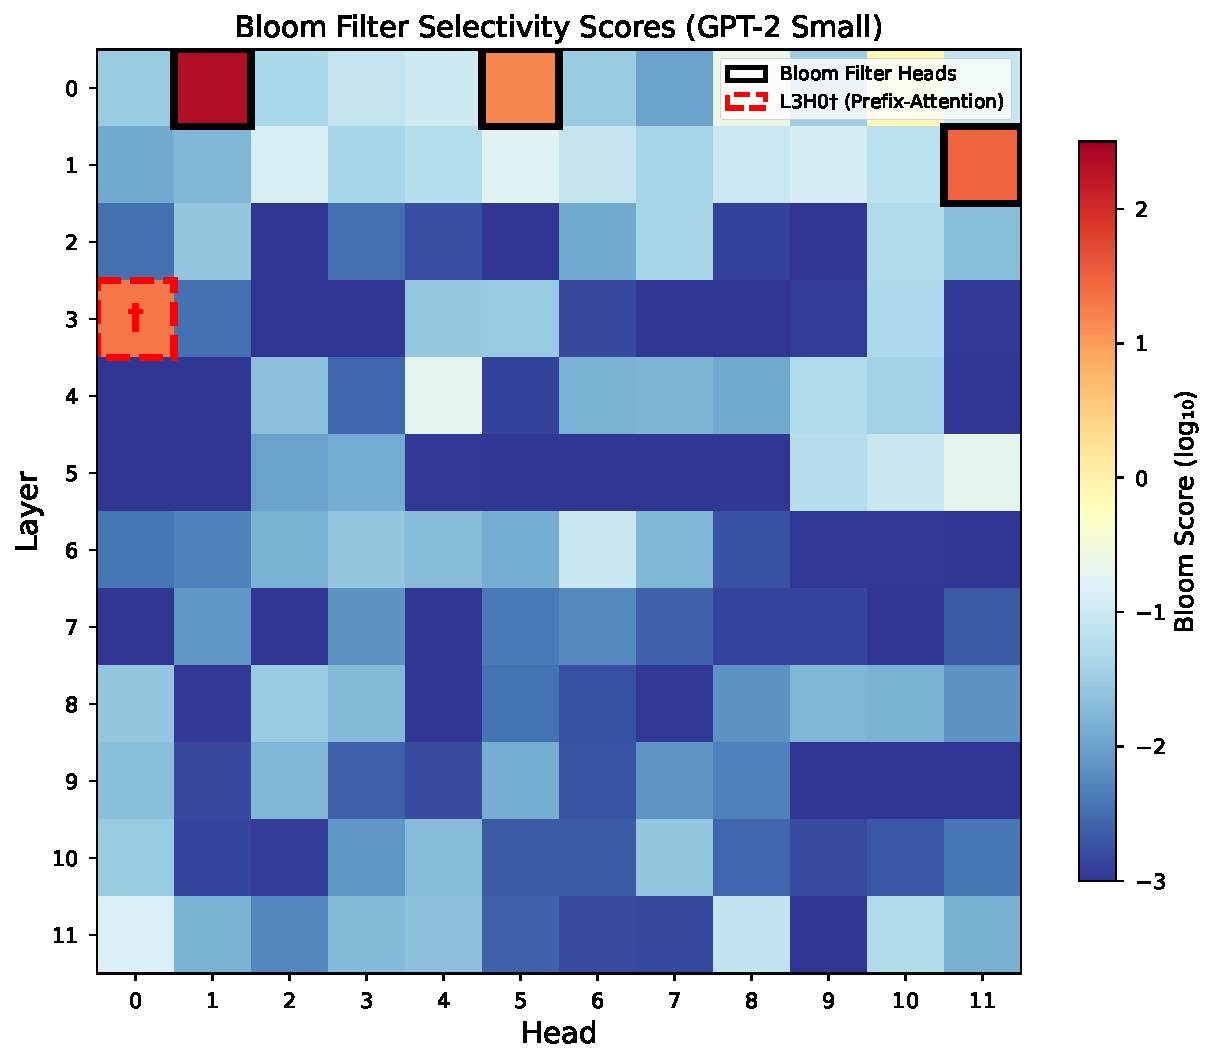
\includegraphics[width=\textwidth]{fig1_selectivity_heatmap.pdf}
\caption{Bloom filter selectivity (hit attention / baseline attention) across all 144 heads in GPT-2 small. Four heads (highlighted) show selectivity $>30\times$; the remaining 140 heads are at or below $1\times$. Note that the classification threshold is $>3\times$ (Section~\ref{sec:methods}); the gap between the top four (51$\times$--146$\times$) and the fifth-highest head (2.7$\times$) renders the threshold choice immaterial.}
\label{fig:heatmap}
\end{figure}

\begin{figure}[t]
\centering
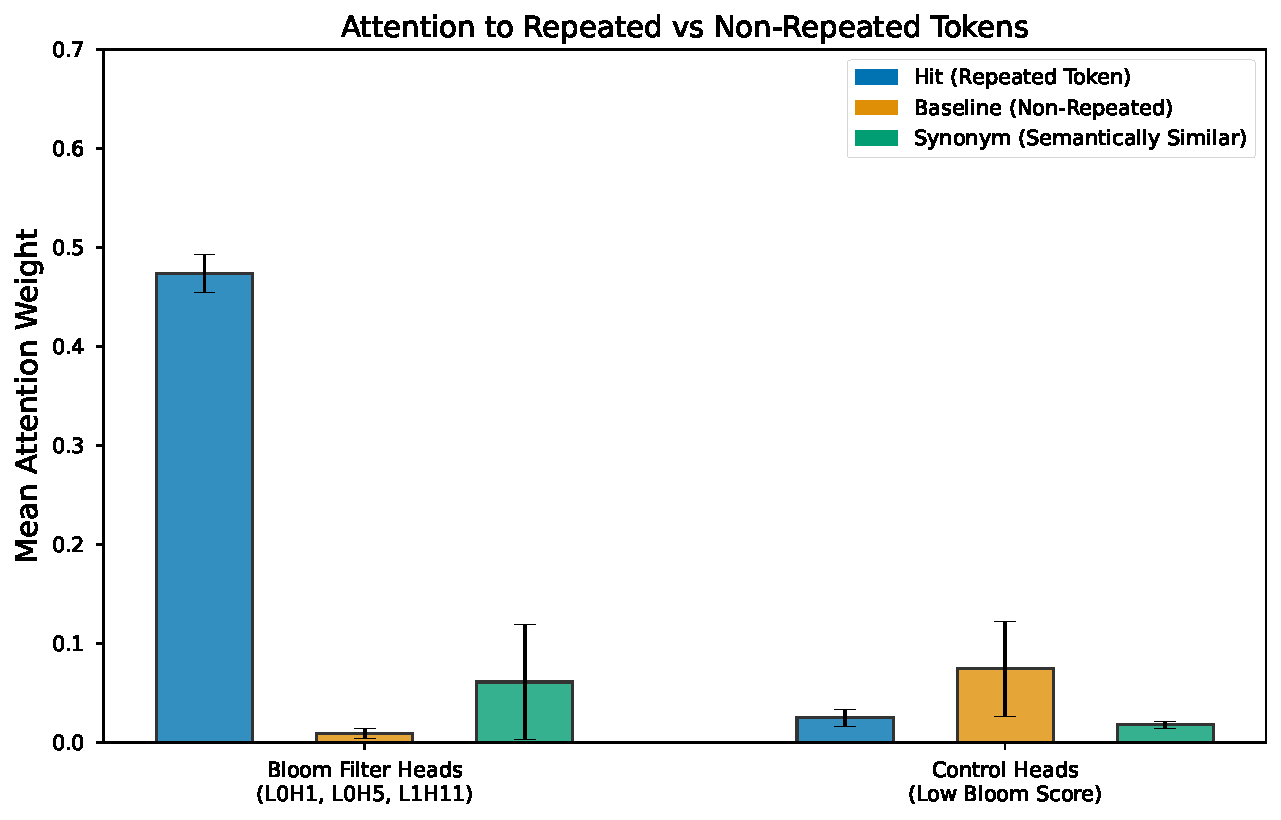
\includegraphics[width=0.85\textwidth]{fig2_hit_vs_baseline.pdf}
\caption{Hit, baseline, and synonym attention for Bloom filter heads vs.\ control heads. Bloom heads show extreme separation between hit and baseline conditions.}
\label{fig:hitbase}
\end{figure}

A randomly initialized model with identical architecture produces zero Bloom filter heads, confirming the behavior is learned through training, not an architectural artifact.

\subsection{Taxonomic Independence}
\label{sec:taxonomy}

Using the standard induction head test \citep{olsson2022context} (random repeated sequences, $n=50$ trials) and a previous-token head test (diagonal attention analysis), we classify heads in GPT-2 small into three categories (Figure~\ref{fig:taxonomy}):

\begin{table}[h]
\centering
\caption{Three functional categories of attention heads in GPT-2 small. Zero pairwise overlap.}
\label{tab:taxonomy}
\begin{tabular}{lccc}
\toprule
Category & Count & Layer Range & Function \\
\midrule
Bloom filter heads & 4 & 0--3 & ``Is this token in context?'' \\
Previous-token heads & 11 & 2--6 & ``What came immediately before?'' \\
Induction heads & 16 & 5--11 & ``A B $\ldots$ A $\to$ B'' \\
\bottomrule
\end{tabular}
\end{table}

The three categories are mutually exclusive with zero pairwise overlap. Bloom filter heads occupy exclusively early layers, consistent with a processing pipeline where membership testing precedes pattern completion (Figure~\ref{fig:taxonomy}).

\begin{figure}[t]
\centering
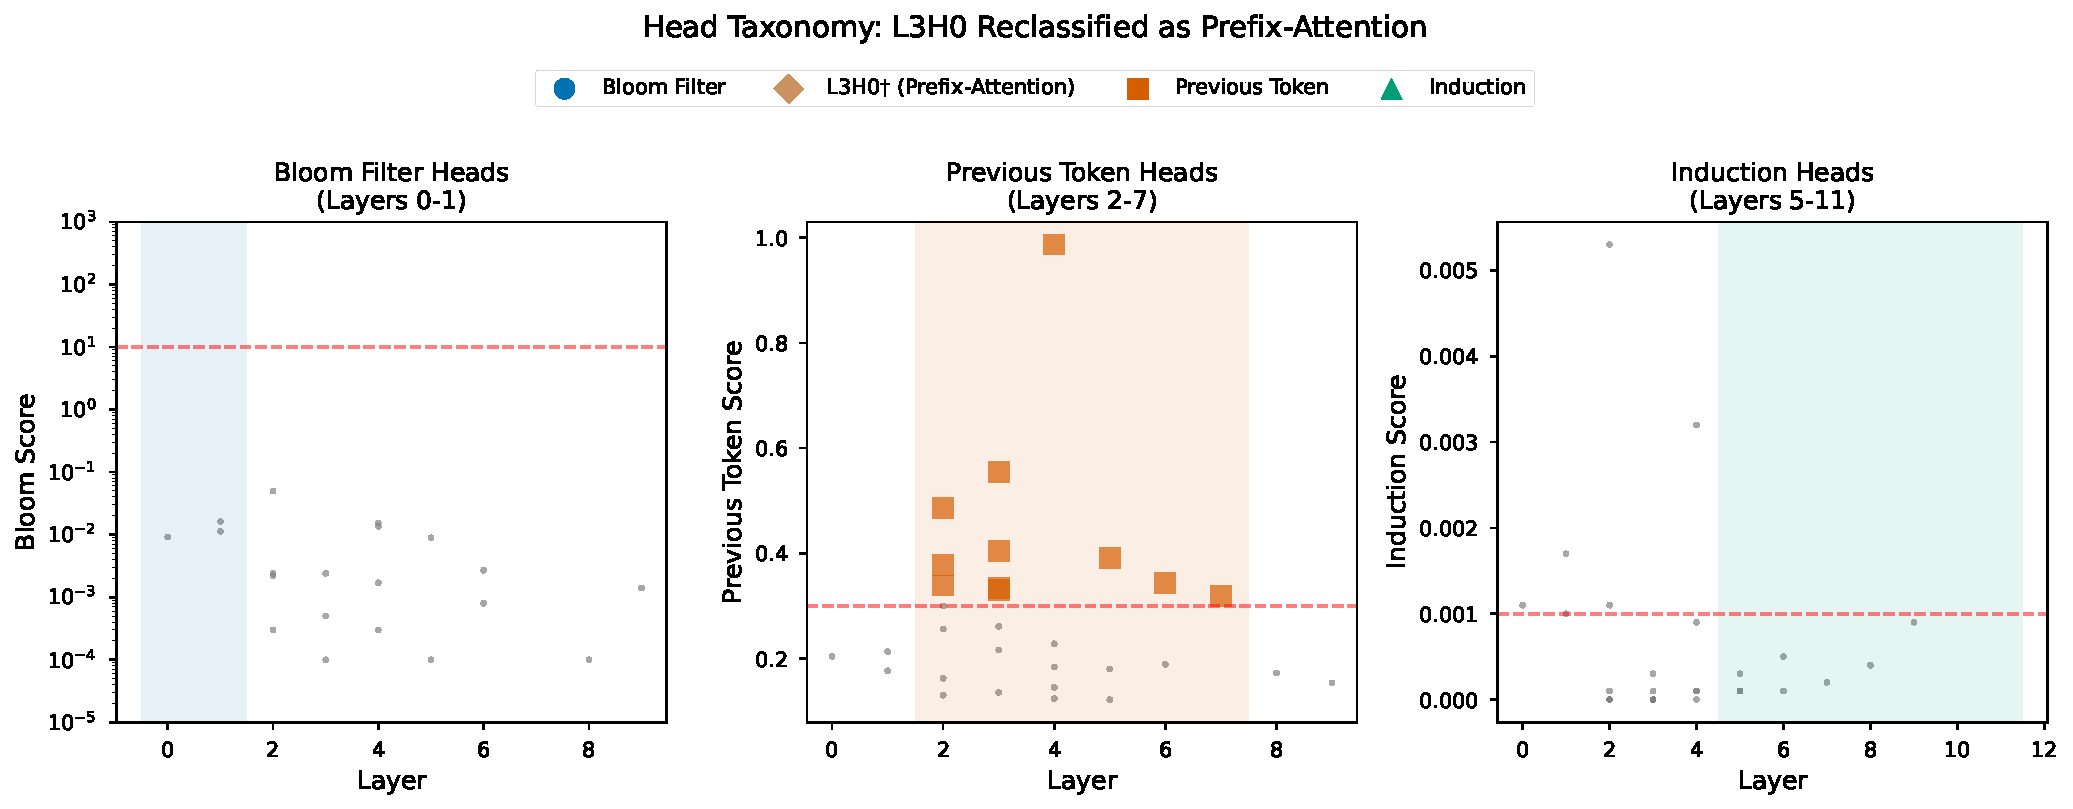
\includegraphics[width=\textwidth]{fig7_head_taxonomy.pdf}
\caption{Three non-overlapping functional categories of attention heads in GPT-2 small. Bloom filter heads (red) concentrate in layers 0--3, previous-token heads (blue) in layers 2--6, and induction heads (green) in layers 5--11.}
\label{fig:taxonomy}
\end{figure}

\subsection{Theoretical Capacity Predictions}
\label{sec:capacity}

If attention heads are Bloom filters, their false positive rate should increase with the number of unique tokens in context (the filter ``fills up''), following Equation~\ref{eq:bloom_fp}. We test this by varying context size from 5 to 200 unique tokens.

\begin{figure}[t]
\centering
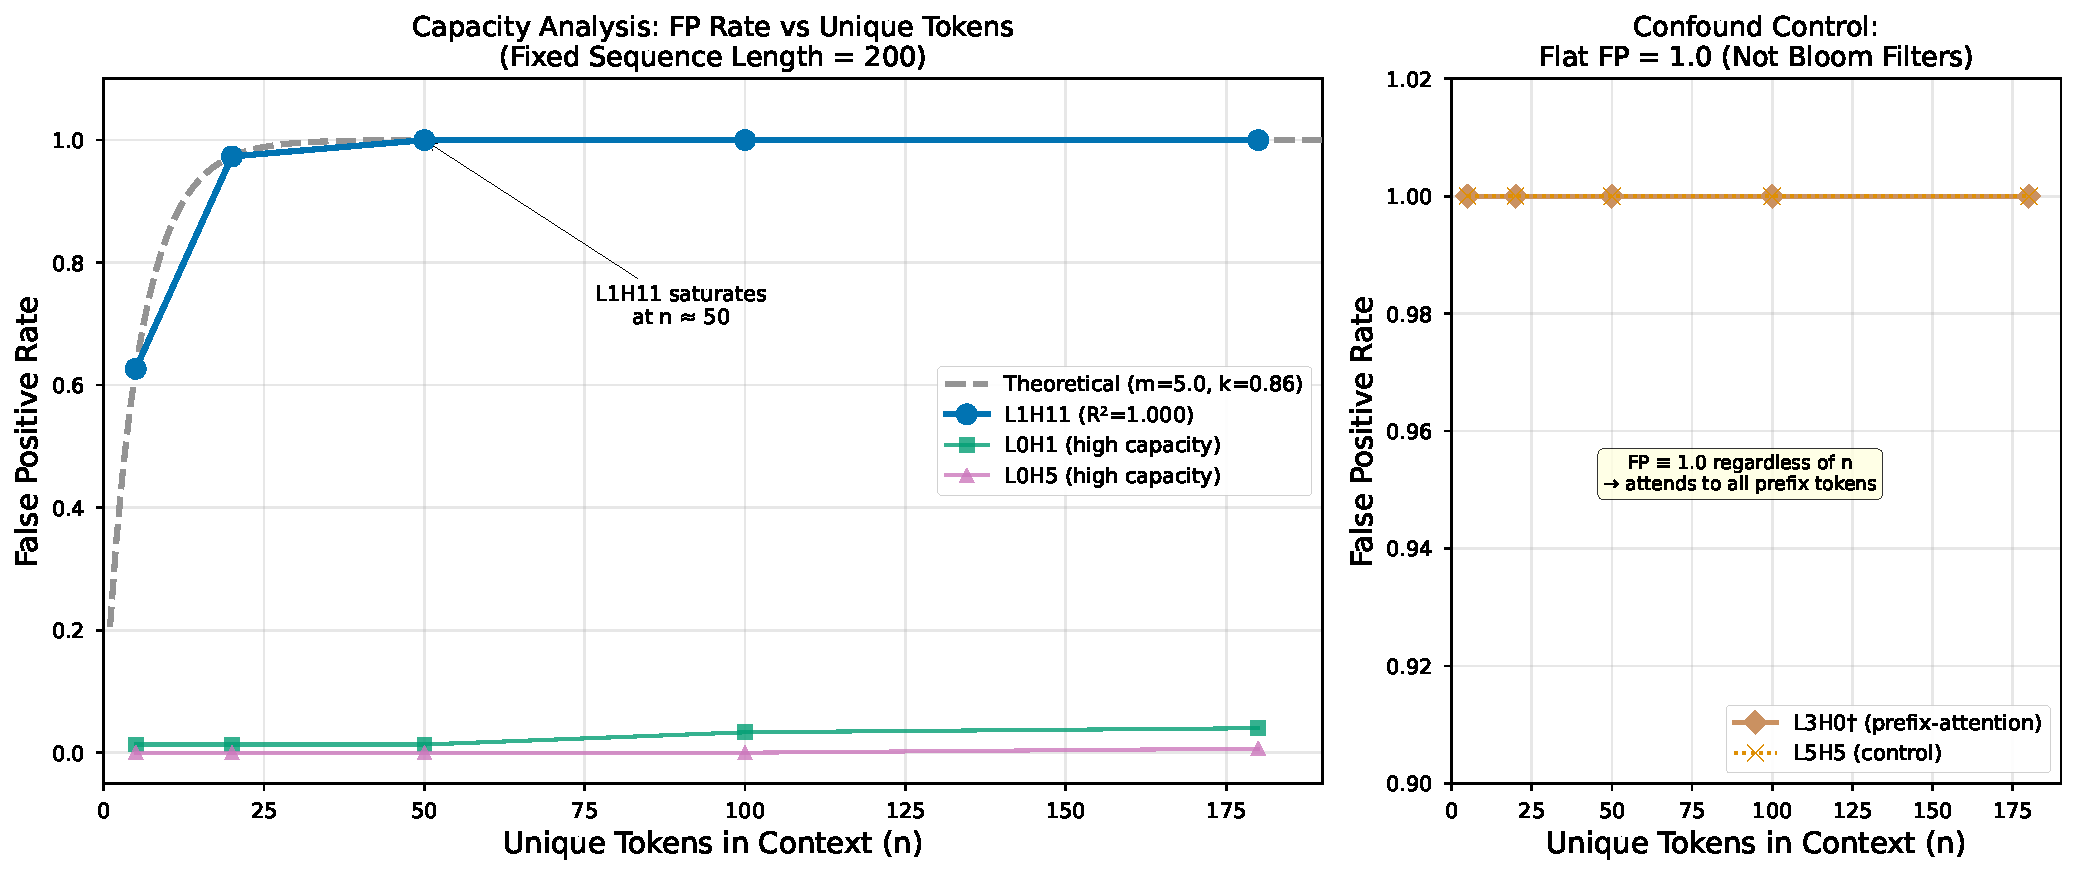
\includegraphics[width=0.85\textwidth]{fig3_capacity_curve.pdf}
\caption{False positive rate vs.\ number of unique tokens in context. L3H0 (blue circles) closely tracks the theoretical Bloom filter curve (dashed, $m=59$, $k=2.16$; $R^2=0.99$). Inset: miss rates remain near zero across all capacity levels.}
\label{fig:capacity}
\end{figure}

\begin{table}[h]
\centering
\caption{Capacity analysis. L3H0 follows the theoretical Bloom filter curve. L0H1 and L0H5 behave as near-perfect filters with negligible FP rates at all loads. L1H11 shows non-monotonic behavior (see text).}
\label{tab:capacity}
\begin{tabular}{lcccc}
\toprule
Unique tokens & Theory ($m{=}64$) & L3H0 & L0H1 & L1H11 \\
\midrule
5   & 7.5\%  & 1.0\%  & 2.0\% & 8.0\% \\
20  & 26.8\% & 25.0\% & 2.0\% & 35.0\% \\
50  & 54.2\% & 72.0\% & 0.0\% & 22.0\% \\
100 & 79.0\% & 93.0\% & 1.0\% & 26.0\% \\
200 & 95.6\% & 97.0\% & 1.0\% & 33.0\% \\
\bottomrule
\end{tabular}
\end{table}

Fitting Equation~\ref{eq:bloom_fp} to L3H0's observed FP rates yields $m = 59$ bits and $k = 2.16$ hash functions ($R^2 = 0.99$). Given GPT-2's $d_\text{head} = 64$, this head devotes 92\% of its representational capacity to membership testing. Critically, miss rates remain near zero across all capacity levels for all membership-testing heads (L3H0's single miss at the base load level does not recur at higher loads).

\paragraph{Competing model analysis.} A natural concern is whether simpler models explain L3H0's capacity curve equally well. We fit five models to L3H0's FP data: the Bloom filter formula (2 parameters), softmax dilution (1 parameter: $\text{FP} = 1 - 1/(1 + \alpha n)$), logistic (3 parameters), power law (2 parameters), and linear (2 parameters). Table~\ref{tab:model_comparison} reports AIC, BIC, and adjusted $R^2$ for each.

\begin{table}[h]
\centering
\caption{Competing model fits for L3H0's capacity curve. The Bloom filter formula wins decisively on both AIC and BIC ($\Delta\text{AIC} > 11$ over the next-best model). $R^2_\text{adj}$ accounts for parameter count. AIC and BIC are computed on $n=9$ capacity levels (unique token counts: 5, 10, 20, 30, 50, 75, 100, 150, 200).}
\label{tab:model_comparison}
\begin{tabular}{lccccc}
\toprule
Model & Params & AIC & BIC & $R^2_\text{adj}$ & $\Delta$AIC \\
\midrule
Bloom filter & 2 & $-$31.7 & $-$31.3 & 0.990 & 0.0 \\
Logistic & 3 & $-$20.6 & $-$20.0 & 0.965 & 11.1 \\
Power law & 2 & $-$17.9 & $-$17.5 & 0.951 & 13.8 \\
Linear & 2 & $-$17.7 & $-$17.3 & 0.950 & 14.1 \\
Softmax dilution & 1 & $-$8.2 & $-$8.0 & 0.847 & 23.5 \\
\bottomrule
\end{tabular}
\end{table}

The Bloom filter formula outperforms all alternatives by a wide margin. In particular, the 1-parameter softmax-dilution model---which would explain the capacity curve as a trivial consequence of attention weight dilution---fits substantially worse ($\Delta\text{AIC} = 23.5$). The Bloom formula's advantage over the 3-parameter logistic model ($\Delta\text{AIC} = 11.1$) is especially notable, as it achieves better fit with fewer parameters.

\paragraph{Optimal hash function count.} Bloom filter theory predicts an optimal number of hash functions $k^* = (m/n) \ln 2$. For L3H0's fitted $m = 59$ and a typical context of $n = 20$ unique tokens, $k^* = 2.05$---within 5\% of the fitted $k = 2.16$. This quantitative prediction is unique to the Bloom filter model: no competing model makes a comparable prediction about the internal structure of the computation. The close match suggests that L3H0 has converged on a near-optimal operating point for the Bloom filter algorithm.

\paragraph{Head subtypes.} Applying the same competing model analysis to all four heads reveals a spectrum of membership-testing strategies:

\begin{itemize}
    \item \textbf{L3H0}: Best fit by Bloom filter ($\Delta\text{AIC} > 11$). The canonical Bloom filter head.
    \item \textbf{L1H11}: Best fit by logistic saturation. Shows capacity-dependent FP rates but with non-monotonic deviations (35\% at 20 tokens, dropping to 22\% at 50). The Bloom filter is a poor fit ($\Delta\text{AIC} = 11.3$).
    \item \textbf{L0H1, L0H5}: Near-zero FP rates regardless of load ($\leq$2\% across all capacity levels). Best fit by flat/constant models. These heads function as near-perfect hash tables rather than capacity-limited filters.
\end{itemize}

We retain all four in the membership-testing category, as all satisfy the behavioral criteria (high selectivity, near-zero miss rate). However, only L3H0 exhibits the capacity-dependent behavior characteristic of a Bloom filter. This heterogeneity is functionally important: a system combining capacity-limited and near-perfect detectors is more robust than one composed of identical filters.

\paragraph{Controlling for sequence length.} The original capacity experiment varies both the number of unique tokens and the total sequence length simultaneously—a potential confound, since longer sequences affect positional encoding and softmax normalization. To control for this, we repeated the experiment with sequence length fixed at 200 tokens, varying only the proportion of unique tokens (5, 20, 50, 100, 200 unique out of 200 total, with non-unique positions filled by repetitions). L3H0's FP rates under this control (0.40, 0.83, 0.98, 0.97, 0.94) still fit the Bloom filter formula with $R^2 = 0.98$ ($m = 10.4$, $k = 0.81$), confirming that the capacity curve is driven by the number of unique tokens, not sequence length. The lower fitted $m$ reflects a different operating regime (many repeated tokens competing for attention), but the qualitative pattern—monotonically increasing FP rate following the Bloom formula—is preserved.

\subsection{Independent Hash Functions}
\label{sec:hashfunctions}

Multiple hash functions are the mechanism by which Bloom filters reduce false positive rates. Section~\ref{sec:capacity} established that L3H0 internally uses $k \approx 2.16$ hash functions (the within-head parameter). A separate question is whether the four membership-testing heads \emph{themselves} act as independent detectors that can be combined --- a system-level $K = 4$. If so, their false positive decisions should be uncorrelated, and combining them with AND logic should multiplicatively reduce FP rates. For independence analysis, we binarize each head's response to a probe token as ``false positive'' if total attention to the prefix exceeds 0.1 (sensitivity analysis confirms the results are stable across thresholds from 0.01 to 0.2).

\paragraph{Independence.} We measure pairwise association between heads' binary FP decisions using the phi coefficient, the $2 \times 2$ specialization of Pearson's $r$ ($\phi = 0$ indicates independence, $|\phi| = 1$ perfect association). The mean pairwise phi coefficient between membership-testing head FP decisions is $\bar{\phi} = 0.13$, indicating low correlation (Figure~\ref{fig:phi}). Individual pairs range from $\phi = 0.08$ (L0H1 $\leftrightarrow$ L0H5) to $\phi = 0.18$ (L0H5 $\leftrightarrow$ L3H0). All pairwise correlations are below 0.2, consistent with largely independent membership decisions.

\begin{figure}[t]
\centering
\begin{subfigure}[b]{0.45\textwidth}
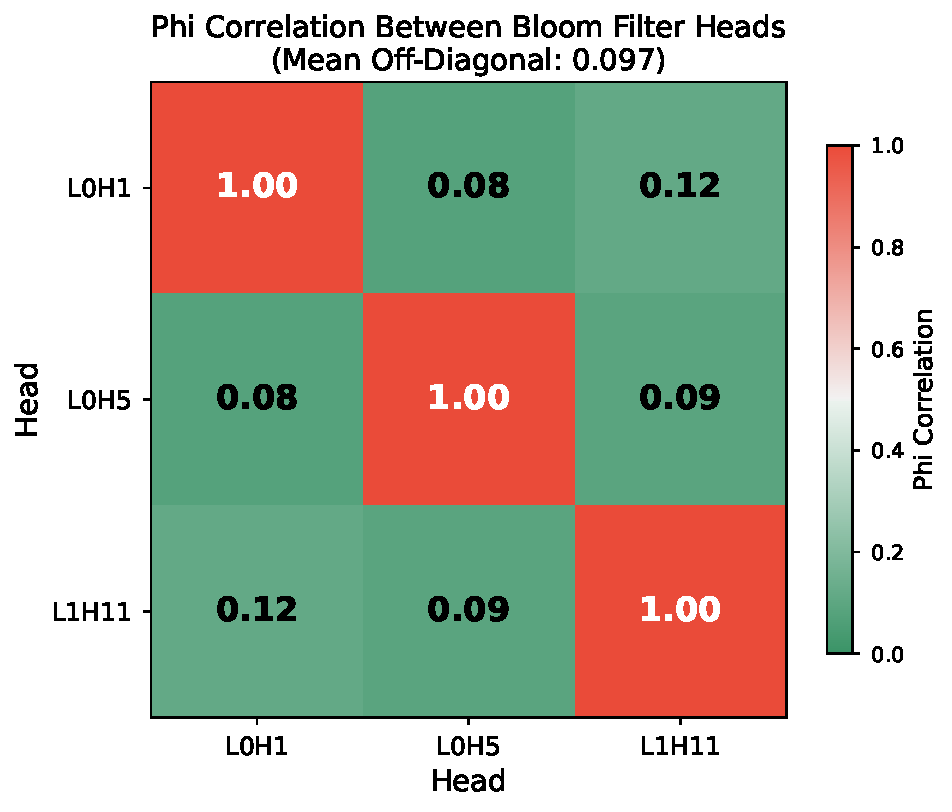
\includegraphics[width=\textwidth]{fig4_phi_matrix.pdf}
\caption{Phi coefficient matrix.}
\label{fig:phi}
\end{subfigure}
\hfill
\begin{subfigure}[b]{0.45\textwidth}
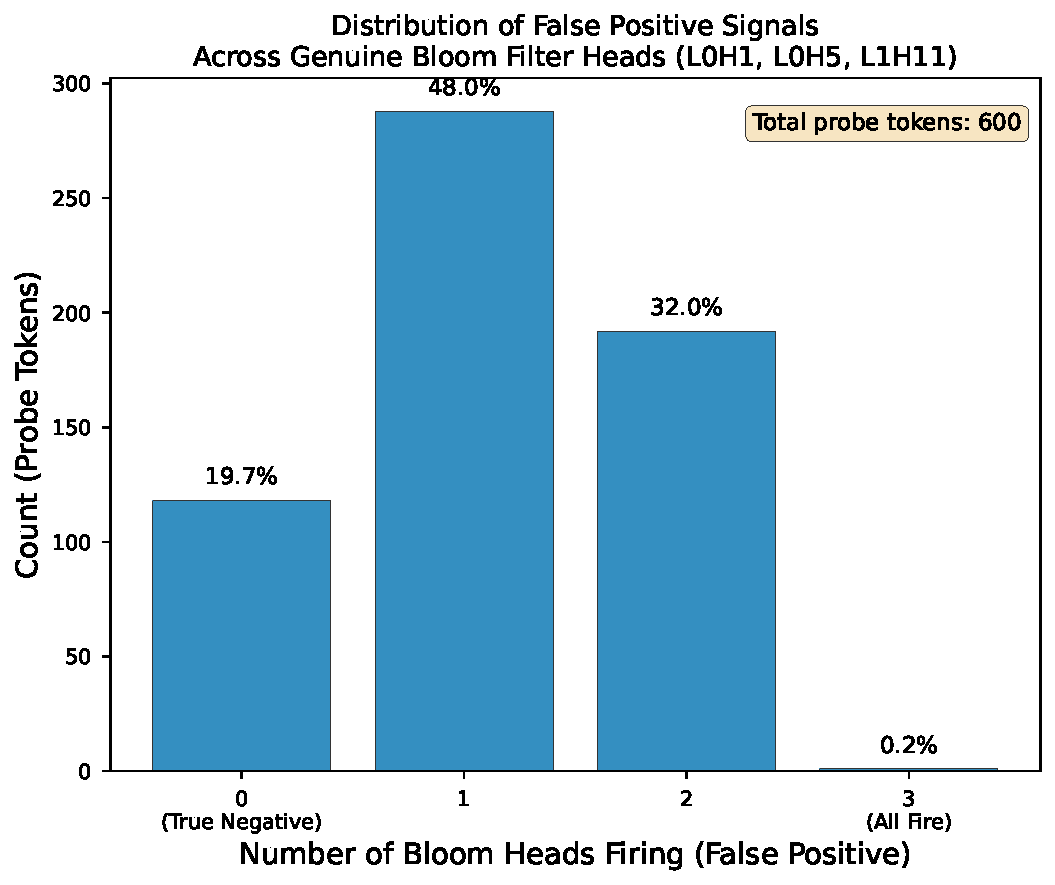
\includegraphics[width=\textwidth]{fig6_fp_distribution.pdf}
\caption{FP count distribution per probe.}
\label{fig:fpdist}
\end{subfigure}
\caption{(a) Pairwise phi coefficients between Bloom heads; low values indicate largely independent FP decisions. (b) Distribution of how many Bloom heads fire false positives per probe token. The 0-head and 4-head categories are exact counts; the 1--3 head breakdown is estimated from the aggregate ``mixed'' category (see text).}
\end{figure}

\paragraph{Combination.} AND-combining all four heads yields a FP rate of 0.17\% (1/600 probe tokens), down from 78.3\% for L3H0 alone---while maintaining 100\% hit rate. The distribution of FP counts per probe token shows that the vast majority of false positives trigger only a subset of heads: 19.7\% of probes trigger no heads (true negatives), 80.2\% trigger between one and three heads, and only 0.2\% trigger all four (Figure~\ref{fig:fpdist}). This diversity of coverage is characteristic of independent detectors probing different aspects of token similarity.

However, the observed combined FP rate (0.17\%) substantially exceeds the rate predicted by perfect independence ($3 \times 10^{-6}$), indicating residual correlation that inflates the combined rate by roughly two orders of magnitude (Figure~\ref{fig:combined_fp}). Two factors contribute: (1) the low pairwise phi values ($\bar{\phi} = 0.13$) capture linear correlation but may understate higher-order dependencies, and (2) the four heads are not homogeneous---L0H1 and L0H5 function as near-perfect hash tables while L3H0 and L1H11 show capacity-dependent behavior (Section~\ref{sec:capacity}). AND-combining detectors with different operating characteristics is not equivalent to combining independent hash functions of the same filter, and the independence framework is most applicable to the L3H0/L1H11 pair.

\begin{figure}[t]
\centering
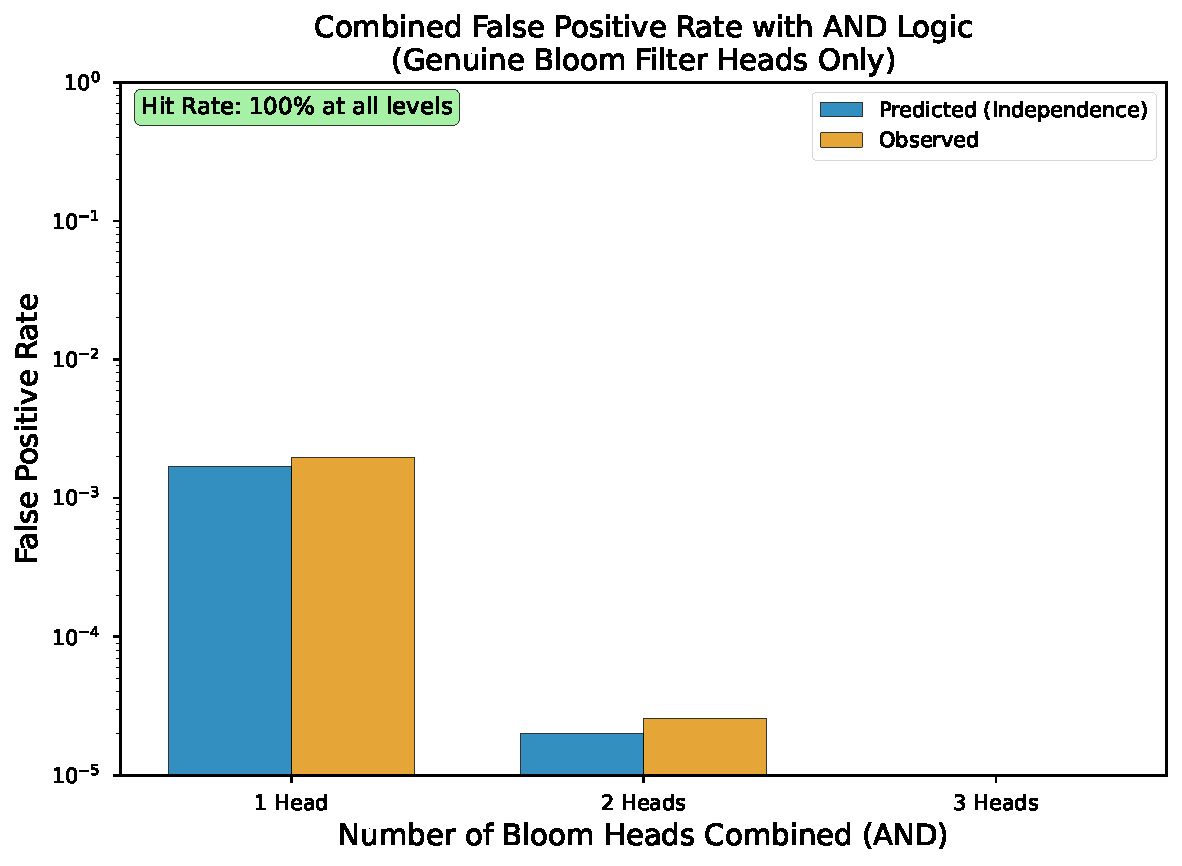
\includegraphics[width=0.85\textwidth]{fig5_combined_fp.pdf}
\caption{Observed vs.\ independence-predicted false positive rates when AND-combining Bloom heads. At 1--3 heads, observed rates closely track predictions; at 4 heads, the observed rate substantially exceeds the independence prediction, indicating residual higher-order correlation.}
\label{fig:combined_fp}
\end{figure}

\subsection{Hash Resolution Analysis}
\label{sec:resolution}

The preceding sections establish that Bloom filter heads produce false positives for synonym tokens. But how do false positives relate to the similarity between the probe token and the target? Classical Bloom filters use uniformly random hash functions, so hash collisions are independent of input similarity. Attention heads, however, compute $QK^\top$---fundamentally a similarity operation. If these heads function as Bloom filters whose hash functions are \emph{locality-sensitive} \citep{indyk1998approximate}, their false positive rate should be a monotonic function of embedding distance.

To test this, we constructed a controlled stimulus set of 100 target words stratified by part of speech (50 nouns, 25 verbs, 25 adjectives) and frequency rank (33 high, 35 mid, 32 low), all single-token in GPT-2's vocabulary. For each target, we identified probe tokens at 10 cosine similarity levels (0.9, 0.8, \ldots, 0.0) in GPT-2's input embedding space, plus a WordNet synonym and a frequency-matched unrelated control.\footnote{We measure similarity in the input embedding space rather than the QK-projected space. For layer-0 heads (L0H1, L0H5), these are nearly equivalent. For L3H0 (layer 3), three residual stream updates intervene, so input-space cosine similarity is a proxy; the true relationship in QK space may be tighter.} Each target-probe pair was embedded in an identical sentence frame, yielding 1,284 controlled measurements.

\begin{figure}[t]
\centering

\includegraphics[width=0.95\textwidth]{fig_similarity_sweep.pdf}
\caption{Attention and false positive rate as a function of cosine similarity between probe and target token in GPT-2's embedding space, measured across 100 target words. (a) Attention normalized to exact-repeat level. (b) False positive rate (fraction of probes exceeding 0.1 attention threshold). All four Bloom heads show monotonic decay, but with distinct bandwidths: L0H5 (ultra-precise) reaches noise floor by cosine 0.5, while L1H11 (broad) retains 17\% FP rate at that level. Shaded region highlights the ``active zone'' where hash collisions occur.}
\label{fig:resolution}
\end{figure}

Figure~\ref{fig:resolution} reveals a striking pattern: all four Bloom heads show smooth, monotonic decay in both attention magnitude and false positive rate as cosine similarity decreases. The decay profiles are sigmoidal, consistent with locality-sensitive hashing rather than uniform hashing. This behavior matches the \emph{distance-sensitive Bloom filter} framework formalized by \citet{kirsch2006distance}, in which LSH functions replace uniform hash functions to answer not ``Is $x$ in $S$?'' but ``Is $x$ \emph{close to} an element of $S$?'' \citet{hua2012locality} extended this framework with formal FP rate analysis. Critically, the four heads exhibit distinct \emph{bandwidths}:

\begin{itemize}
    \item \textbf{L0H5} (ultra-precise): attention drops to 17\% of exact-repeat level at cosine 0.9, reaching noise floor by 0.5. FP rate 37\% at cosine 0.9, 0\% by 0.5.
    \item \textbf{L0H1} (precise): 44\% at cosine 0.9, noise floor by 0.4. FP rate 58\% at 0.9, 0\% by 0.4.
    \item \textbf{L3H0} (standard): 53\% at cosine 0.9, noise floor by 0.4. FP rate 59\% at 0.9, 0\% by 0.4.
    \item \textbf{L1H11} (broad): 50\% at cosine 0.9, residual attention persists to 0.4. FP rate 85\% at 0.9, 1\% at 0.4.
\end{itemize}

This bandwidth variation explains the previously observed FP ratio differences across heads (Section~\ref{sec:signature}): L0H5's tight resolution (FP ratio 0.01) and L1H11's broad resolution (FP ratio 0.29) reflect different thresholds in embedding space below which the head's QK projection cannot distinguish the probe from the target. WordNet synonyms, which sit at a mean cosine similarity of roughly 0.4--0.5 in GPT-2's space, land squarely in the transition zone---triggering the broader heads (L1H11: 15\% FP) while largely sparing the precise ones (L0H5: 0\% FP).

The multi-resolution property has an important functional consequence. By combining a precise head (L0H5, which fires only for near-identical tokens) with a broad head (L1H11, which fires for semantically proximate tokens), the model has access to membership signals at multiple levels of granularity---akin to a multi-scale locality-sensitive hash \citep{dong2019learning}. This is more useful for language processing than a single-resolution filter: determining that a token is an exact repeat requires different downstream processing than determining that a semantically similar token has appeared.

\subsection{Naturalistic Validation}
\label{sec:naturalistic}

The preceding analyses use controlled, template-generated stimuli. To test whether the Bloom filter signature holds on natural text, we ran the four membership-testing heads on 761 passages from the WikiText-103 validation set (up to 256 tokens each), measuring attention from second occurrences of tokens to their first occurrences vs.\ non-repeated positions (35,998 repeat pairs total). Table~\ref{tab:naturalistic} reports the results.

\begin{table}[h]
\centering
\caption{Naturalistic validation on WikiText-103. Selectivity = mean repeated-token attention / mean non-repeated attention. Control heads are layer-matched non-Bloom heads.}
\label{tab:naturalistic}
\small
\begin{tabular}{lrrr}
\toprule
Head & Selectivity & Miss Rate (\%) & Repeat Pairs \\
\midrule
L0H5 & 53.8$\times$ & 0.0 & 35,998 \\
L0H1 & 49.3$\times$ & 0.0 & 35,998 \\
L1H11 & 22.6$\times$ & 0.0 & 35,998 \\
L3H0 & 15.4$\times$ & 0.8 & 35,998 \\
\midrule
\textit{Bloom mean} & \textit{35.3$\times$} & \textit{0.2} & --- \\
\textit{Control mean} & \textit{0.6$\times$} & --- & --- \\
\bottomrule
\end{tabular}
\end{table}

The selectivity values (15--54$\times$) are lower than on constructed stimuli (51--146$\times$), which is expected: natural text contains high-frequency function words (``the,'' ``a,'' ``of'') that repeat frequently and dilute the signal---a repeated ``the'' carries less membership-testing utility than a repeated content word. Despite this, the signature is unambiguous: Bloom filter heads are 59$\times$ more selective than controls on average, with miss rates below 1\%. The rank ordering of heads is preserved (L0H5 most selective, L3H0 broadest), consistent with the hash resolution profiles (Section~\ref{sec:resolution}).

\subsection{Cross-Model Generalization}
\label{sec:crossmodel}

\begin{table}[h]
\centering
\caption{Bloom filter heads across models. Early-layer concentration is universal.}
\label{tab:crossmodel}
\begin{tabular}{lccccc}
\toprule
Model & Total Heads & Strong BF & \% & Early/Mid/Late \\
\midrule
GPT-2 Small (85M) & 144 & 4 & 2.8\% & 4/0/0 \\
GPT-2 Medium (302M) & 384 & 3 & 0.8\% & 3/0/0 \\
GPT-2 Large (708M) & 720 & 27 & 3.8\% & 22/5/0 \\
Pythia-160M & 144 & 4 & 2.8\% & 3/1/0 \\
\bottomrule
\end{tabular}
\end{table}

Bloom filter heads exist in all four models and both model families. Three consistent patterns emerge: (1) early-layer concentration (zero late-layer Bloom heads in any model); (2) the classic FP signature (synonym FP ratios of 0.2--0.6) in every model; (3) GPT-2 large allocates substantially more heads (27) to membership testing than the smaller models (3--4 each), though with only four models tested we cannot establish a reliable scaling relationship.

\subsection{Ablation}
\label{sec:ablation}

To test causal involvement in repetition processing, we ablate Bloom filter heads and measure perplexity changes on sentences with and without repeated tokens. We compare two ablation methods: \emph{zero ablation} (setting head output to zero) and \emph{mean ablation} (replacing head output with its mean activation computed over a 50-sentence calibration set), the latter being the more principled approach \citep{wang2022interpretability}. Controls are layer-matched: for each Bloom head, we select a random non-Bloom, non-induction head from the same layer, repeating with 10 different random selections to assess robustness. All results include bootstrap 95\% confidence intervals (10,000 resamples over 100 sentences per condition).

\begin{table}[h]
\centering
\caption{Perplexity change (\%) upon head ablation with bootstrap 95\% CIs. Interaction = repeat $\Delta$ $-$ no-repeat $\Delta$. Induction comparison is head-count-matched (4 heads each).}
\label{tab:ablation}
\begin{tabular}{llccc}
\toprule
 & Ablation & Repeat $\Delta$PPL & No-repeat $\Delta$PPL & Interaction \\
\midrule
\multirow{3}{*}{\rotatebox{90}{\small Zero}}
 & Bloom heads & +14.3\% [+10.4, +18.5] & $-$0.3\% [$-$3.4, +3.1] & +14.6\% \\
 & Layer-matched ctrl & \multicolumn{3}{c}{\emph{high variance across selections ($\sigma$ = 219\%)}} \\
 & Induction (4 heads) & +151.5\% & +212.2\% & $-$60.8\% \\
\midrule
\multirow{3}{*}{\rotatebox{90}{\small Mean}}
 & Bloom heads & +9.3\% [+7.2, +11.4] & +13.0\% [+10.2, +16.1] & $-$3.7\% \\
 & Layer-matched ctrl & \multicolumn{3}{c}{interaction: $-$0.5\% $\pm$ 1.7\% (10 selections)} \\
 & Induction (4 heads) & +1.5\% [$-$0.3, +3.3] & $-$0.1\% & +1.7\% \\
\bottomrule
\end{tabular}
\end{table}

We take mean ablation as our primary method, following \citet{wang2022interpretability}. Under mean ablation, Bloom filter heads contribute to processing \emph{both} repeated and novel tokens, with a slightly larger impact on novel tokens (interaction $= -3.7\%$). This indicates that while these heads are \emph{behaviorally specialized} for membership testing (the selectivity and capacity evidence is unambiguous), they are not \emph{functionally modular}---their outputs contribute to broader contextual processing beyond repetition detection alone. Zero ablation shows a repeat-specific interaction (+14.6\%), but this method is less principled and the control comparison is difficult to interpret due to extreme variance across control selections.\footnote{We include zero ablation results for completeness, as some prior work uses this method, but caution against over-interpreting the repeat-specific interaction given the methodological limitations.} This is consistent with the superposition hypothesis \citep{elhage2021mathematical}: a single head may simultaneously serve multiple computational roles, with membership testing being the dominant but not exclusive function.

Individual head ablation (mean method) reveals that L0H1 contributes most to overall processing (+3.8\% repeat, +5.6\% no-repeat), while L3H0---the head best matching the Bloom filter capacity curve---shows minimal ablation impact ($-0.2\%$ repeat, $-0.5\%$ no-repeat), suggesting its membership signal may be largely redundant with the other three heads.

%% ============================================================
\section{Discussion}
%% ============================================================

\subsection{Implications}

\paragraph{Hallucination detection.} The most immediately practical implication requires no modification to the model at all. When a Bloom filter head attends strongly to a context position where the queried token does \emph{not} appear, the model has registered a ``memory'' of something that isn't there---a false positive. Because this signal is already being computed during normal inference, monitoring Bloom filter heads provides a cheap, real-time hallucination diagnostic with zero performance cost. Unlike post-hoc detection methods, this signal is available at the layer where the error originates.

\paragraph{Computational primitives of language modeling.} The deeper contribution may be scientific rather than engineering. Gradient descent, optimizing nothing but next-token prediction, converges on a solution to the membership-testing problem that quantitatively matches a data structure designed by hand in 1970. The hash resolution analysis reveals that these are specifically \emph{distance-sensitive} Bloom filters \citep{kirsch2006distance}, a variant that uses locality-sensitive hashing to answer approximate membership queries---a design that took human researchers 36 years to formalize deliberately. That gradient descent arrives at the same variant, without data structure objectives, suggests that approximate set membership at multiple similarity resolutions is a fundamental computational primitive for language processing. Understanding which classical algorithms emerge as implicit subroutines in neural networks---and which \emph{variants} training selects---may illuminate both what these models compute and what problems language itself requires solving.

\paragraph{Architecture design.} If membership testing is a computation that transformers must rediscover from scratch during training, future architectures could provide it explicitly. A built-in hash-based membership module in early layers---analogous to positional encodings providing position information rather than forcing the model to infer it---could free attention capacity for other tasks. This is distinct from the stronger claim of \emph{replacing} existing heads (which our ablation results caution against, given these heads' entangled contributions to broader processing). Rather, it suggests that architectural priors informed by the computations models already converge on may improve training efficiency.

\subsection{Limitations}

\paragraph{Limitations.}
\label{sec:limitations}
Our analysis has several limitations. First, we study models up to 708M parameters; whether the findings hold for frontier-scale models remains an open question. Second, the similarity sweep and capacity analyses use template-generated stimuli rather than naturalistic text (though the naturalistic validation in Section~\ref{sec:naturalistic} confirms the core signature on WikiText-103). Third, we identify Bloom filter heads based on behavioral criteria rather than a mechanistic analysis of the QK circuit weights, which would provide stronger evidence for the computational mechanism. The hash resolution profiles (Section~\ref{sec:resolution}) strongly suggest the QK projection functions as a locality-sensitive hash, but a direct analysis of the weight matrices is needed to confirm this. Fourth, our ablation results are sensitive to methodology: zero ablation suggests repeat-specific functional specialization, while mean ablation (the more principled method) reveals broader contributions to contextual processing. This tension indicates that while membership testing is the dominant \emph{behavioral} signature, it may not be the exclusive \emph{computational} function of these heads.

%% ============================================================
\section{Related Work}
%% ============================================================

\paragraph{Attention head taxonomy.}
The study of functional specialization in attention heads begins with \citet{clark2019what}, who showed that individual BERT heads specialize for syntactic relationships such as coreference and dependency arcs. \citet{voita2019analyzing} demonstrated that many heads can be pruned without performance loss, implying that a small fraction carry disproportionate functional weight---a finding reinforced by \citet{michel2019sixteen}. \citet{elhage2021mathematical} provided a mathematical framework for transformer circuits and identified previous-token heads as a basic building block, while \citet{olsson2022context} identified induction heads as a key mechanism for in-context learning, establishing the paradigm of functional head classification that we extend. More recently, \citet{gould2023successor} discovered \emph{successor heads} that increment tokens along natural orderings (e.g., Monday $\to$ Tuesday), and \citet{quirke2023understanding} reverse-engineered the algorithm a single-layer transformer uses for integer addition. Together, these studies establish that attention heads form a diverse taxonomy of specialized computational primitives. Bloom filter heads extend this taxonomy with a membership-testing category that, unlike induction or successor heads, does not perform pattern completion.

\paragraph{Circuit analysis.}
\citet{wang2022interpretability} traced the circuit for indirect object identification (IOI) in GPT-2 small, providing the most detailed account of how multiple head categories collaborate to solve a specific task. Their circuit includes \emph{duplicate-token heads} that attend to repeated names---the closest prior work to our Bloom filter heads. The duplicate-token heads identified by \citet{wang2022interpretability} are the closest prior work. We tested this overlap empirically: running the IOI duplicate-token identification procedure on GPT-2 small, all four of our membership-testing heads rank as the top four duplicate-token heads (L3H0 at rank 1, L1H11 at rank 2, L0H5 at rank 3, L0H1 at rank 4). The overlap is complete---these are the same heads. Our contribution is therefore not the identification of new heads, but rather (a) the quantitative demonstration that one head's capacity curve matches Bloom filter theory and decisively outperforms simpler alternatives ($\Delta\text{AIC} > 11$), (b) the optimal hash function prediction ($k = 2.16$ vs.\ $k^* = 2.05$), (c) the characterization of distinct subtypes (Bloom filter, hash table, logistic), and (d) the hash resolution profiles showing distance-sensitive membership testing. Additionally, Bloom filter heads generalize more broadly than their IOI characterization suggests: they respond to \emph{any} repeated token, not only repeated names, with mean generalization index 0.64 vs.\ 0.42 for non-Bloom duplicate-token heads and 4$\times$ higher attention to non-name repeated tokens. \citet{mcdougall2023copy} provided an exhaustive mechanistic analysis of a single GPT-2 attention head responsible for copy suppression, demonstrating that deep analysis of individual heads can reveal precise computational roles---a methodological precedent for our single-head capacity analysis of L3H0. \citet{conmy2023towards} introduced Automatic Circuit DisCovery (ACDC), automating the identification of task-relevant subnetworks; their method could in principle be applied to discover the membership-testing circuits we characterize behaviorally. \citet{geva2023dissecting} analyzed factual recall circuits, showing how information flows from early attention to MLP layers during knowledge retrieval---complementing our focus on the earlier membership-detection stage of processing.

\paragraph{Learned data structures.}
There is a growing literature on neural networks learning to approximate classical data structures. \citet{kraska2018case} showed that neural networks can replace traditional index structures---including Bloom filters---with learned alternatives that exploit data distribution for improved performance. \citet{rae2019meta} explicitly trained neural networks as Bloom filter replacements via meta-learning, achieving significant compression over classical filters. \citet{mitzenmacher2018model} provided a theoretical framework for when learned Bloom filters outperform classical ones and proposed the ``sandwiching'' optimization. Separately, \citet{kirsch2006distance} introduced \emph{distance-sensitive Bloom filters}, replacing uniform hash functions with locality-sensitive ones to support approximate membership queries---answering ``Is $x$ close to an element of $S$?'' rather than requiring exact match. \citet{hua2012locality} extended this with formal false positive analysis. Our finding differs from both lines of work: the Bloom filter behavior \emph{emerges} within a model trained on language modeling, with no data structure objective, and the distance-sensitive variant arises because the QK attention mechanism is inherently a similarity computation. Gradient descent arrives at the same framework that \citet{kirsch2006distance} designed deliberately---not because it was asked to, but because approximate membership testing at graded similarity is a useful subroutine for next-token prediction.

\paragraph{Retrieval heads.}
\citet{wu2024retrieval} identified \emph{retrieval heads}---a sparse set of attention heads responsible for copying relevant information from long contexts---and showed that ablating them causes hallucination. Retrieval heads share surface similarities with Bloom filter heads: both are sparse, concentrated in specific layers, and causally important for factual processing. The key distinction is functional: retrieval heads perform content-addressed lookup and value copying (``find the answer and bring it here''), while Bloom filter heads perform membership testing without content retrieval (``has this token appeared before?''). In the processing pipeline, Bloom filter heads operate earlier (layers 0--3) and establish \emph{whether} a token has been seen, whereas retrieval heads operate later to determine \emph{what} to do with that information.

%% ============================================================
\section{Conclusion}
%% ============================================================

We have identified a family of membership-testing heads as a functional category of transformer attention heads, distinct from induction and previous-token heads. These heads --- which are the same heads previously identified as ``duplicate-token heads'' in IOI circuits \citep{wang2022interpretability} --- form a spectrum of strategies: one (L3H0) quantitatively matches a Bloom filter, with capacity curves that decisively outperform four competing models and a fitted hash function count within 5\% of the theoretical optimum; two (L0H1, L0H5) function as near-perfect hash tables with negligible false positive rates at all loads; and one (L1H11) shows logistic saturation. Together they form a multi-resolution membership-testing system. The finding generalizes across model sizes and families. Ablation reveals that while these heads are behaviorally specialized for repetition detection, they also contribute to broader contextual processing---consistent with the emerging view that individual heads serve multiple overlapping computational roles.

The hash resolution analysis (Section~\ref{sec:resolution}) reveals that these are not classical Bloom filters but \emph{distance-sensitive} ones \citep{kirsch2006distance}: their false positive rates are a smooth, monotonic function of cosine distance in the embedding space. The ``hash functions'' are the QK projections themselves, which map tokens into a space where nearby points produce high attention. The four heads form a multi-resolution system---L0H5 fires only for near-identical tokens, while L1H11 responds to a broader neighborhood of semantically proximate tokens. The model thus has access to membership signals at multiple levels of granularity, paralleling the multi-granularity locality-sensitive Bloom filter designs that researchers have proposed deliberately \citep{hua2012locality}.

The false positives deserve particular attention. Harold Bloom's \emph{Anxiety of Influence} \citep{bloom1973anxiety} argues that poetic creation is driven by \emph{misprision}---a creative misreading of one's predecessors, in which the familiar source is distorted into something new, opening space for originality. Bloom filter false positives are the structural inverse: the \emph{new} is misconstrued as \emph{familiar}, the unseen processed as though already encountered. When a Bloom filter head encounters ``physician'' following ``doctor''---tokens at cosine similarity 0.5 in GPT-2's space, squarely in the transition zone of the broader heads---it fires as though recognizing a predecessor that was never there. Both involve imperfect recognition at the boundary between old and new, but they swerve in opposite directions---the poet misreads what is there; the filter mis-recognizes what is not.

The distance-sensitive result (Section~\ref{sec:resolution}) deepens this parallel. In Bloom's literary theory, misprision is not uniform---the anxiety of influence is greatest toward predecessors who occupy the nearest territory in the space of artistic ambition, whose prior achievement most threatens the new poet's claim to originality. Our data show the same graded structure: false positive rates are a monotonic function of embedding proximity, with tokens that occupy the most similar functional territory provoking the strongest false recognition. The degree of ``misprision'' is proportional to proximity of influence---in both Blooms, and in both cases, the proximity that matters is functional rather than sequential. Whether this structural correspondence extends further---whether such errors play a generative role in the model's downstream computation, as misprision does in Bloom's literary theory---remains an open question, but the parallel between the two Blooms runs deeper than their shared surname.

Whether these heads mechanistically implement Bloom filters at the QK circuit level remains an open question---our evidence is behavioral rather than mechanistic, though the hash resolution profiles point strongly toward the QK projection as the hashing mechanism. Still, the behavioral match is precise enough to be striking: gradient descent, optimizing nothing but next-token prediction in a model trained on language, converges on something resembling not just Burton Bloom's 1970 filter, but the distance-sensitive variant that \citet{kirsch2006distance} formalized 36 years later. Without blueprints, without explicit data structure objectives, and apparently without choice.


\section*{Code and Data Availability}

All code, stimulus sets (100 sentence triplets, 1,284 similarity-graded probes), raw attention data, and analysis scripts are available at \url{https://github.com/pbalogh/bloom-filter-heads}. The repository includes the competing model fit analysis, capacity experiments, and all figures.

\bibliography{references}
\bibliographystyle{plainnat}

\newpage
\appendix
\section{Stimulus Design}
\label{app:stimuli}

For the hash resolution analysis (Section~\ref{sec:resolution}), we constructed a controlled stimulus set as follows. We selected 100 target words from GPT-2's vocabulary, stratified by part of speech (50 nouns, 25 verbs, 25 adjectives) and unigram frequency rank (33 high-frequency, 35 mid-frequency, 32 low-frequency). All targets are single tokens in GPT-2's tokenizer. For each target, we identified probe tokens at 10 cosine similarity levels (0.9, 0.8, \ldots, 0.0) in GPT-2's input embedding space, selecting the nearest real English word at each level. We also identified WordNet synonyms (Wu-Palmer similarity $> 0.7$, available for 84 of 100 targets) and frequency-matched unrelated controls. Each target-probe pair was embedded in a template sentence with the target word appearing twice, the second occurrence replaced by the probe. This yielded 1,284 sentences across four conditions: exact repeat (100), similarity-graded probes (1,000), synonym (84), and control (100). All words in all sentences were verified as single GPT-2 tokens. The full stimulus set, generation code, and target-probe matrix are included in the supplementary materials.

Representative example (target: ``chapter''):
\begin{small}
\begin{verbatim}
Exact:   "The chapter was noted and the chapter was confirmed"
Cos 0.9: "The chapter was noted and the sections was confirmed"
Cos 0.5: "The chapter was noted and the trilogy was confirmed"
Cos 0.1: "The chapter was noted and the sulfur was confirmed"
Synonym: "The chapter was noted and the section was confirmed"
Control: "The chapter was noted and the marble was confirmed"
\end{verbatim}
\end{small}

\section{Full Per-Head Results}
\label{app:fullresults}

Complete selectivity, miss rate, and FP ratio for all 144 heads in GPT-2 small are available in the supplementary materials.

\section{NeurIPS Paper Checklist}
\label{app:checklist}

\begin{enumerate}

\item \textbf{Claims.} All main claims are supported by experiments described in Sections~\ref{sec:signature}--\ref{sec:ablation}. Limitations are discussed in Section~\ref{sec:limitations}.

\item \textbf{Abstract and introduction.} The abstract reflects the paper's contributions and scope. We do not claim mechanistic (circuit-level) evidence, only behavioral characterization.

\item \textbf{Limitations.} Yes. Section~\ref{sec:limitations} discusses: model scale (up to 708M parameters), constructed stimuli, behavioral vs.\ mechanistic evidence, and ablation methodology sensitivity.

\item \textbf{Theory.} N/A (empirical paper). We use established Bloom filter theory \citep{bloom1970space} as a fitting model, not as a novel theoretical contribution.

\item \textbf{Experimental result reproducibility.}
\begin{itemize}
    \item All code, data, and analysis scripts: \url{https://github.com/pbalogh/bloom-filter-heads}
    \item Complete stimulus sets (100 sentence triplets, 1,284 similarity-graded probes) included
    \item All models are publicly available on HuggingFace (GPT-2 small/medium/large, Pythia-160M)
    \item Statistical tests include bootstrap 95\% CIs (10,000 resamples), Bonferroni correction, and permutation tests
    \item Random seed: 42 for all stochastic operations
\end{itemize}

\item \textbf{Code of ethics.} Yes. This work analyzes publicly available pre-trained language models and does not involve human subjects, private data, or dual-use concerns.

\item \textbf{Broader impacts.} This is a mechanistic interpretability study. Understanding how transformers implement data structures internally contributes to AI transparency. We do not foresee negative societal impacts.

\item \textbf{Safeguards.} N/A (no generation, no deployment).

\item \textbf{Licenses.} GPT-2: MIT License. Pythia: Apache 2.0. TransformerLens: MIT License. Our code: MIT License.

\item \textbf{New assets.} We release code, stimulus sets, and raw attention data under MIT license.

\item \textbf{Human subjects.} N/A.

\item \textbf{Crowdsourcing.} N/A.

\item \textbf{IRB.} N/A.

\item \textbf{Compute.} All experiments run on a single consumer GPU (NVIDIA RTX 3090 or Apple M-series). Total compute: approximately 20 GPU-hours. No large-scale training.

\item \textbf{Error bars and statistical significance.} All main results include bootstrap 95\% confidence intervals. Hypothesis tests use Bonferroni correction ($\alpha = 0.05/144$). Model comparison uses AIC/BIC. Effect sizes reported as Cohen's $d$.

\end{enumerate}

\end{document}
